\documentclass[10pt]{article}
\usepackage[T1]{fontenc}
\usepackage[utf8]{inputenc}
\usepackage{mathptmx}
\usepackage{amsmath,amssymb}
\usepackage{graphicx,booktabs,array,enumitem,xcolor,fancyhdr,titlesec,caption,microtype}
\usepackage[paperwidth=8.5in,paperheight=11in,textwidth=5.5in,textheight=9in,top=1in,headsep=0.25in,headheight=12pt]{geometry}
\setlength{\parindent}{0pt}
\setlength{\emergencystretch}{3em}
\setlength{\parskip}{5.5pt}
\setlength{\tabcolsep}{3pt}
\renewcommand{\arraystretch}{1.15}
\titleformat{\section}{\large\scshape}{\thesection}{0.6em}{}
\titleformat{name=\section,numberless}{\large\scshape}{}{0em}{}
\titleformat{\subsection}{\normalsize\bfseries}{\thesubsection}{0.6em}{}
\titlespacing*{\section}{0pt}{12pt plus 3pt minus 2pt}{5pt plus 1pt}
\titlespacing*{\subsection}{0pt}{8pt plus 2pt minus 1pt}{3pt plus 1pt}
\captionsetup{font=small,labelfont=bf,labelsep=colon,justification=justified}
\pagestyle{fancy}
\fancyhf{}
\fancyhead[L]{\small CSE 516 Major Project, Milestone 4 (Ahmedabad University)}
\fancyfoot[C]{\thepage}
\renewcommand{\headrulewidth}{0.4pt}
\fancypagestyle{plain}{\fancyhf{}\fancyfoot[C]{\thepage}\renewcommand{\headrulewidth}{0pt}}
\setlist[itemize]{leftmargin=1.4em,itemsep=2pt,topsep=2pt,parsep=0pt}
\begin{document}
\thispagestyle{plain}
\noindent\rule{\textwidth}{4pt}\par\vspace{0.2in}
{\fontsize{17}{21}\selectfont\scshape\raggedright Can a Deep Temporal Causal Posterior Be Trusted? Error-Controlled Edge Selection for Rhino\par}\vspace{0.22in}
{\bfseries Het Patel}\par\vspace{2pt}
Ahmedabad University, Ahmedabad, India (student ID AU2440266)\par
CSE 516, Probabilistic Graphical Models. Individual project, Theoretical AI track.\par
Group g12\_th\_conditional-ind-graphs\_ind. Milestone 4, final report.\par
\vspace{0.12in}
\begin{center}{\large\scshape Abstract}\end{center}\vspace{-6pt}
\begin{list}{}{\setlength{\leftmargin}{0.5in}\setlength{\rightmargin}{0.5in}\setlength{\topsep}{0pt}}\item[]
\small Rhino (Gong et al., ICLR 2023) learns non-linear temporal causal graphs with instantaneous effects and history-dependent noise, and it returns a probability for every possible edge. The paper judges the output by AUROC and F1 against a known graph. It does not ask whether the probabilities can be trusted, that is, whether a user who keeps the edges above a chosen level gets the share of wrong edges that the probabilities promise. This report states that question as a small idea and a plan: take the finished Rhino models as they are, read the exact edge probabilities, select edges under an error budget, and measure the realised share of wrong edges against the budget. For any selected set, the share of wrong edges equals the promised error plus the overconfidence of the posterior on that set. As a first test I use 500 finished Rhino runs from M3. The posterior is saturated: 9.4\% of the entries have p above 0.999 and 23.3\% of them are not edges. With a budget of 0.01 the realised share is 0.306 [0.277, 0.335] (95\% CI over 120 datasets). Temperature scaling lowers the calibration error from 0.200 to 0.039 but does not restore the promise. A cutoff learned on other datasets brings the share close to the budget for budgets of 0.1 to 0.3, at the price of power, and it does not carry over to DREAM3. These are early results on one benchmark family. They show where the idea holds and where it does not.
\end{list}
\section{Introduction}
A causal graph learned from data is only useful if someone can act on it. A biologist who reads a gene graph, or a neuroscientist who reads a brain connectivity graph, will follow up the edges one by one. What they need is a statement such as: at most one in ten of these edges is wrong. Most methods return one graph and give no such statement. Papers measure quality by comparing against a known true graph. A user in practice has no true graph.

Rhino (Gong et al., 2023) is a Bayesian method. It models non-linear effects, instantaneous effects and history-dependent noise in time series, and it learns a distribution q(G) over graphs. This distribution looks like exactly what a user needs, because it gives a probability for every possible edge. But the paper scores the probabilities only through AUROC and through a graph rounded at 0.5. In M3 I saw a warning sign. On Netsim the AUROC of Rhino falls from 0.989 to 0.939 while the training goes on, and the validation likelihood falls from -31.5 to -76.1, while the F1 rises. The model becomes more sure without becoming more right.

\textbf{Question.} Can the edge probabilities of a deep temporal causal posterior be used to select edges with a stated error budget, and if not, what is the cheapest way to repair this?

\textbf{What this report offers.} It is a small idea with a plan and a first test, not a new causal discovery method.

\begin{itemize}
\item \textbf{An idea.} Treat Rhino's probabilities as a promise about the share of wrong edges, and check the promise. The one formal fact I use is an identity: the share of wrong edges equals the promised error plus the overconfidence on the selected set (Section 2).
\item \textbf{A plan that trains nothing.} Read the exact edge probabilities from the saved weights of the M3 runs, calibrate them with one temperature or one cutoff learned on other datasets, and compare the realised share of wrong edges with the budget. I analyse 500 finished runs: 440 synthetic, 10 Netsim and 50 DREAM3 (Section 12).
\item \textbf{First evidence, with limits.} The raw posterior is saturated and overconfident. Temperature scaling improves the probability scores but not the promise. A cutoff learned on other datasets helps for moderate budgets, costs power, and does not carry over to DREAM3 (Sections 12 and 15).
\end{itemize}
\textbf{Scope and history.} In M1 and M2 I studied uGLAD for conditional independence graphs. On 31 October 2026 I changed the base paper to Rhino. M3 reproduced the experiments of the Rhino paper with the authors' code. This report uses the M3 runs as raw material. No model was trained again for M4. What I add is the question, a small idea with a plan, and a first test of the posterior on those runs. I reused from M1 and M2 the habit of fair baselines and of stating what did not reproduce.

\textbf{Why it matters, and what it costs.} If the posterior could be trusted, a user could choose a budget and read off the graph. The first evidence says this works only after a repair that needs labelled graphs from similar data, and only for moderate budgets. That is a useful and a limited answer, and I state both sides in Sections 14 and 15.

\textbf{How the report is organised.} It follows the order of the talk: what Rhino is and what its paper shows (Section 3), the gap the paper leaves (Section 2.1), then the idea, why it is logical, why it matters, the plan, the KPIs and what I expect (Sections 2, 11 and 12).

\section{Problem Formulation}
This section gives the idea behind the project and the plan to test it. It is short on purpose. It follows the order of the talk: the gap, the idea, why it is logical, why it matters, the plan, and what I expect. I do not claim a theory here. The one formal fact I use is an identity that holds for any selected set.

\subsection{The gap}
The Rhino paper checks its output against a known true graph, with AUROC and with the F1 of a graph rounded at 0.5. A real user has no true graph. They will follow up the top edges one by one, in the lab or in the clinic, and they want to know how many will turn out to be wrong. That question has an answer only if the probabilities mean what they say. A probability is calibrated if, among the entries scored 0.9, about nine in ten are real edges.

There is a warning sign. In M3 the validation likelihood of Rhino falls during training, as the paper's own Figure 8 shows, and the AUROC falls with it while the F1 rises (Section 1). I see four reasons to suspect the probabilities, and none of them is established. (1) The objective rewards likelihood and not the quality of edge probabilities. (2) The posterior is a product of independent factors and so ignores dependence between edges. (3) Long training with sparsity and acyclicity penalties can push the logits to extremes. (4) The posterior comes from one training run on small data and nobody checks it against the truth. The study tests whether these matter.

\subsection{Our idea}
Take Rhino as given and ask whether its edge probabilities can be used to select edges under an error budget. Let $p_e\in[0,1]$ be the probability of edge entry $e=(l,i,j)$, meaning an edge from variable $i$ to variable $j$ at lag $l$, and let $y_e\in\{0,1\}$ be the unknown truth. Given the probabilities and a budget $\alpha$, choose a set $S$ of entries that finds as many true edges as possible, while the expected share of wrong edges in $S$ stays at most $\alpha$. At use time no true graph is available. Labels are used only on calibration datasets, which do have true graphs. I call this selective temporal causal discovery. It is a way of using a causal discovery method, not a new one.

\subsection{Why it is logical}
Write $\mathrm{FDP}(S)$ for the share of wrong edges in $S$, and $a(S)=\frac{1}{|S|}\sum_{e\in S}(1-p_e)$ for the error that the posterior promises on $S$. Then, for any non-empty $S$,

\begin{equation}\mathrm{FDP}(S)\;=\;a(S)\;+\;o(S),\qquad o(S)=\frac{1}{|S|}\sum_{e\in S}(p_e-y_e).\end{equation}
The term $o(S)$ is the overconfidence of the posterior on the chosen set. The identity is one line of algebra, because both sides are one minus a mean (Appendix A). It says what to look for: the promise fails exactly where the posterior is overconfident on what it selects. If the probabilities are calibrated, the overconfidence averages to zero and the classical Bayesian false discovery rule of Newton et al. (2004) controls the expected share of wrong edges. A second fact, also standard, limits any repair that only rescales the probabilities: a strictly increasing map of p keeps the order of the entries, so it keeps AUROC and the top-k sets. Both facts are stated and checked in Appendix A. I make no claim that they are new.

\subsection{Why it matters}
Think of a gene network with a hundred candidate edges. Every edge that is followed costs an experiment. If the probabilities are trustworthy, a user can choose a budget, for example at most one wrong edge in ten, and get the longest list that respects it. If they are not, the user cannot choose how many edges to follow, and is misled without knowing it.

\subsection{Our plan}
The plan has three steps and trains nothing. I keep the finished Rhino models from M3. (1) Read the exact edge probabilities from the saved weights. (2) Calibrate them, with one temperature or one cutoff on the log-odds, both learned on other datasets that have a known graph. (3) Select the edge set with the Bayesian false discovery rule. The selection itself costs a sort. Sections 7 and 8 give the details. Section 11 lists the KPIs and why each is used. The key one is the realised share of wrong edges against the budget, because it tests the promise directly, where the user reads the list.

\subsection{What I expect}
\begin{figure}[!ht]\centering
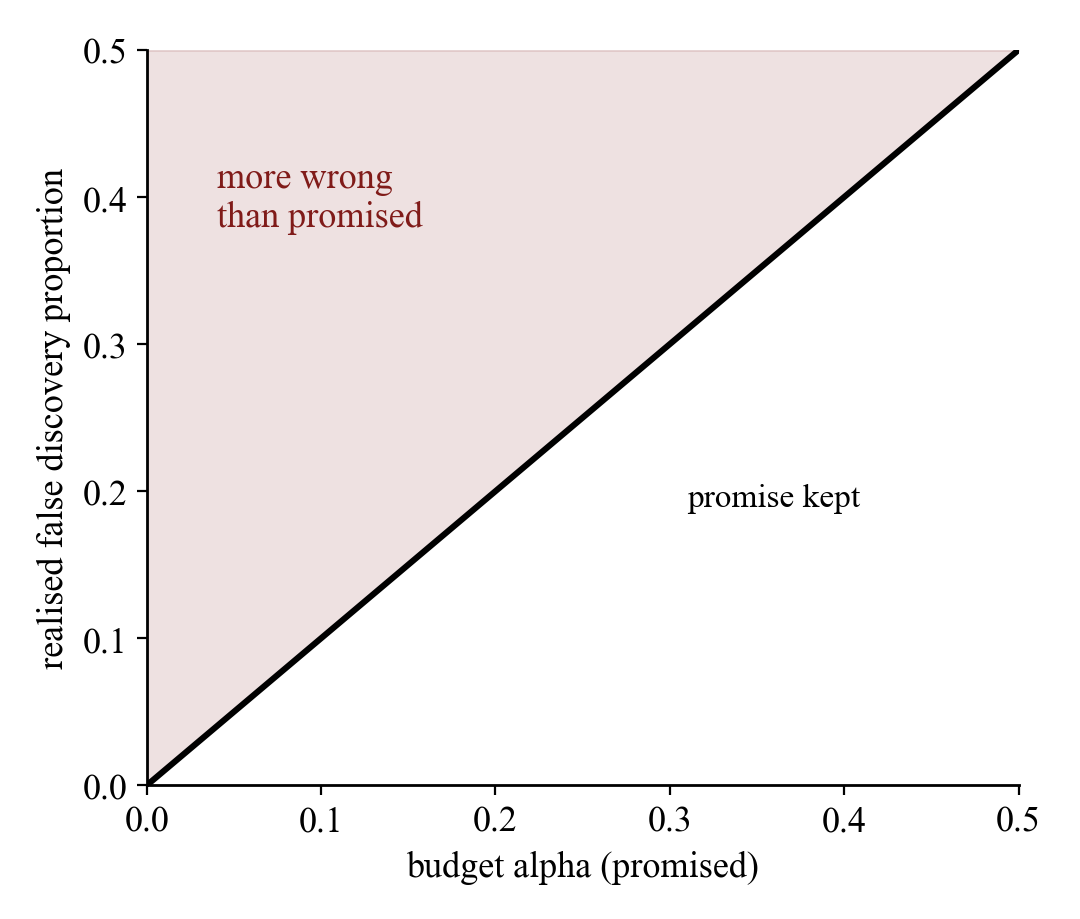
\includegraphics[width=0.48\textwidth]{figures/slide_target.png}
\captionsetup{type=figure}\caption*{\textbf{Figure 1:} The target, as a schematic and not as a result. On the diagonal the promise is kept. Above it there are more wrong edges than promised.}
\end{figure}
I expect the raw posterior to land above the diagonal. I expect a repair to bring it near the diagonal for moderate budgets, at a price in power, and I do not expect the repair to transfer to real data without a check. These are expectations that the data can contradict, and Section 12 reports where they do. The wording of the five expectations is below. H5 was added after I saw the temperature result, so it is exploratory.

\begin{itemize}
\item \textbf{H1.} The raw posterior breaks its own budget: the realised share of wrong edges is clearly above $\alpha$.
\item \textbf{H2.} Temperature scaling, fitted on other datasets, lowers Brier score, log-loss and ECE, and brings the realised share close to $\alpha$.
\item \textbf{H3.} The graph that maximises the expected F1 under the calibrated posterior beats a threshold of 0.5 and comes close to the oracle threshold.
\item \textbf{H4.} The temperature fitted on synthetic data transfers to Netsim and DREAM3, or if not, the promise degrades as expected when the calibration data differ from the new data.
\item \textbf{H5 (exploratory, added after H2).} A cutoff on the log-odds, learned on other datasets so that the pooled share of wrong edges is at most $\alpha$, brings the realised share close to $\alpha$.
\end{itemize}
\subsection{Benefits and costs}
\textbf{Benefits if it works.} A user gets an error budget in the units they care about. The method needs no change of the model and no retraining, and it costs seconds. \textbf{Costs and limits.} It needs labelled graphs from similar data. The promise is an average over datasets, not a guarantee for one dataset. Calibration cannot repair a weak ranking. A budget that is too strict selects nothing. I measure each of these costs.

\section{Background}
\textbf{What we want to learn, and why it is hard.} We observe several variables over time, for example gene expression or signals from brain regions, and we want to know which variable drives which and after how many time steps. The Rhino paper names three features of real series that make this hard. Effects are non-linear. With slow sampling, everything that happens between two measurements is folded into one time step, which creates instantaneous effects. And the noise is not fixed: how much a variable scatters can depend on its own past. Granger-type methods, including the neural ones (Khanna \& Tan, 2019; Tank et al., 2018; Nauta et al., 2019), assume no instantaneous effects and a fixed noise distribution. VAR-LiNGAM (Hyvärinen et al., 2010) and DYNOTEARS (Pamfil et al., 2020) handle instantaneous effects but are linear with fixed noise. PCMCI+ (Runge, 2020) handles both kinds of effect with conditional independence tests, but does not model the noise. Rhino (Gong et al., 2023) handles all three features at once.

\textbf{Rhino as a structural equation model.} The value of variable $i$ at time $t$ is given by

\begin{equation}X_{i,t}=f_i\big(\mathrm{Pa}_i^{<t},\mathrm{Pa}_i^{t}\big)+g_i\big(\mathrm{Pa}_i^{<t},\varepsilon_{i,t}\big).\end{equation}
The function $f$ is a neural network, and $g$ is a conditional spline flow that reshapes the noise $\varepsilon$ as a function of the lagged parents. So the noise can grow or shrink with the history. The graph is a tensor of shape $[L+1,D,D]$. Slice 0 holds the instantaneous edges and the slices 1 to $L$ hold the lagged edges (Gong et al., 2023). The paper proves that the graph is identifiable under conditions on $f$ and $g$ (Gong et al., 2023, Theorem 1). I use this result and I do not re-prove it.

\textbf{Variants.} Rhino+g uses Gaussian noise that does not depend on history. Rhino+s uses a spline noise that does not depend on history. These variants test single ideas of the model, and I use them to see how the posterior depends on the noise model.

\textbf{Calibration.} A probability forecast is calibrated if events forecast with probability p happen in about a fraction p of the cases. I use the Brier score, the log-loss, the expected calibration error with 10 equal-width bins (Guo et al., 2017; Naeini et al., 2015) and reliability diagrams. Temperature scaling divides the logit by one parameter $\tau$ fitted on held-out data (Guo et al., 2017).

\textbf{False discovery rate.} The false discovery proportion of a list is the fraction of wrong items. Benjamini and Hochberg (Benjamini \& Hochberg, 1995) control its expectation with p-values. With posterior probabilities, the posterior expected FDP of a list is the mean of (1 $-$ p) over the list, and the largest list with a given value is the Bayesian FDR selection (Newton et al., 2004).

\textbf{What the base paper shows.} The paper uses three benchmarks: 160 synthetic datasets (five per setting, 75\% built to mismatch Rhino's own configuration), the DREAM3 gene networks and the Netsim brain-region simulations. Its main results are below. The numbers are copied from the tables of the paper (Gong et al., 2023) and are not my runs. My own M3 reproduction of the same experiments is in the last row.

\begin{table}[!ht]\centering
\captionsetup{type=table}\caption*{\textbf{Table 1:} Main results of the Rhino paper (Gong et al., 2023)}
\footnotesize
\begin{tabular}{>{\raggedright\arraybackslash}p{1.50in}>{\raggedright\arraybackslash}p{1.19in}>{\raggedright\arraybackslash}p{1.19in}>{\raggedright\arraybackslash}p{1.27in}}\toprule
\textbf{Benchmark and measure} & \textbf{Rhino} & \textbf{Comparison in the paper} & \textbf{Reading} \\ \midrule
Synthetic, temporal F1, true lag 2 (5, 10, 20, 40 nodes) & 0.59, 0.49, 0.39, 0.37 & Rhino with lag 1: 0.34, 0.28, 0.25, 0.20 & Best or close to best. History-dependent noise helps the lagged graph. A longer assumed lag (3) costs little \\
DREAM3, AUROC of the summary graph, five networks & 0.685, 0.680, 0.664, 0.585, 0.567 (Rhino+g higher on the last two) & eSRU: 0.660, 0.629, 0.627, 0.557, 0.550 & Rhino or Rhino+g is highest on all five networks \\
Netsim, AUROC of the summary graph & 0.990 & cMLP 0.930, TCDF 0.910 & Without instantaneous effects Rhino drops to 0.930, so modelling them matters \\
M3, Netsim, my reproduction with the authors' code & 0.987 & Not rerun & Close to the paper's 0.990 \\
\bottomrule\end{tabular}
\par\vspace{3pt}{\footnotesize Rhino+g is Rhino with Gaussian noise that does not depend on history. The paper reports the DREAM3 AUROC of Rhino and Rhino+g for the networks above; I show the Rhino value first.}
\end{table}
All of these measures compare the output with a known true graph. They say how accurate Rhino is. They do not say whether its probabilities can be trusted, and this is the gap that Section 2 takes up.

\section{Related Work}
\textbf{Temporal causal discovery.} PCMCI+ (Runge, 2020) uses conditional independence tests with lags and instantaneous effects. DYNOTEARS (Pamfil et al., 2020) uses continuous optimisation with an acyclicity penalty (Zheng et al., 2018). VAR-LiNGAM (Hyvärinen et al., 2010) uses non-Gaussianity. Nonlinear Granger methods use neural networks (Khanna \& Tan, 2019; Tank et al., 2018; Nauta et al., 2019). Rhino (Gong et al., 2023) adds history-dependent noise and a posterior over graphs. A survey is in (Assaad et al., 2022). These works evaluate by F1, SHD or AUROC against a known graph.

\textbf{Uncertainty and calibration of causal graphs.} Jabbari et al. (2017) show that bootstrap estimates of edge probabilities are not guaranteed to be calibrated, and calibrate them after the fact for causal Bayesian networks. AVICI (Lorch et al., 2022) reports the expected calibration error of its edge probabilities, for static graphs. PRCD-MAP (Shan \& Zhou, 2026) calibrates how much to trust an outside prior in the causal discovery objective. It does not study the final edge probabilities or the error of the selected edges (I read the abstract and a summary of the paper, not the full text). I did not find a study of the calibration of Rhino's posterior.

\textbf{Error control for edges.} MMPC-p (Guillen Pegueroles et al., 2018) controls the false discovery rate of a structure learner for time series with p-values. Bayesian FDR (Newton et al., 2004) and the Benjamini-Hochberg procedure (Benjamini \& Hochberg, 1995) are the classical tools. Learn then Test (Angelopoulos et al., 2021) gives a general way to choose a parameter, such as my cutoff, so that a risk is controlled with a finite-sample guarantee. My cutoff rule has no such guarantee, and I say so in Section 15. \textbf{Position.} To my knowledge, I did not find earlier work that audits the posterior of a deep temporal causal model for error control. The search was limited, and I make no claim of being first.

\section{SOTA Positioning}
I follow the course loop: identify, understand, compare, validate, reposition.

\begin{table}[!ht]\centering
\captionsetup{type=table}\caption*{\textbf{Table 2:} The anchor work and this project}
\footnotesize
\begin{tabular}{>{\raggedright\arraybackslash}p{0.80in}>{\raggedright\arraybackslash}p{2.17in}>{\raggedright\arraybackslash}p{2.25in}}\toprule
\textbf{Item} & \textbf{Rhino (Gong et al., Microsoft Research, ICLR 2023) (Gong et al., 2023)} & \textbf{This project} \\ \midrule
Problem & Causal discovery from time series with non-linear effects, instantaneous effects and history-dependent noise & Can the posterior of such a model be used to select edges with a stated error budget? \\
Representation & SEM over time. Graph tensor [L+1, D, D]. Variational posterior q(G) & Same posterior, plus a selection layer: forecasts p, a set S, a budget $\alpha$ \\
Learning & ELBO, augmented Lagrangian for acyclicity, Gumbel-softmax samples & Rhino weights from M3. One temperature, or a cutoff, learned on other datasets \\
Inference & Edge probabilities, rounded graph, treatment effects & Exact marginal p\_e from the logits. Bayesian FDR set, learned cutoff \\
Evaluation & F1, SHD, AUROC, treatment effect RMSE. Synthetic, DREAM3, Netsim & ECE, Brier, log-loss, realised FDP versus budget, power. Same data \\
Findings & Best or close to best on synthetic data and real benchmarks & First test: the posterior is saturated. Calibration alone does not keep the promise. A learned cutoff comes close for moderate budgets \\
Limits & Cost. Hand-tuned settings. No uncertainty on the graph quality & Needs labelled data. Average guarantee. Loses power. No transfer to DREAM3 \\
\bottomrule\end{tabular}
\end{table}
\textbf{Compare and validate.} In M3 the F1 of Rhino was the highest of the six methods on synthetic data, with a significant gain over PCMCI+ at 5 and 10 nodes only. That comparison measures accuracy. This report measures trust. The two disagree: among the Rhino variants, the one with the lowest F1 (Rhino+s) is the only one whose raw probabilities are close to their promise (Section 12.6).

\textbf{Reposition.} My M1 position was a study of uGLAD with a Microsoft Research anchor on causal order. After the change of base paper, my anchor is Rhino. I do not claim a better causal discovery algorithm, and I do not claim a new theory. The project is an idea for checking the trust of a published method, a plan to test it, and a first test on finished runs, with its limits. I did not survey work after the Rhino paper beyond the search in Section 4.

\section{Graphical Representation}
\begin{figure}[!ht]\centering
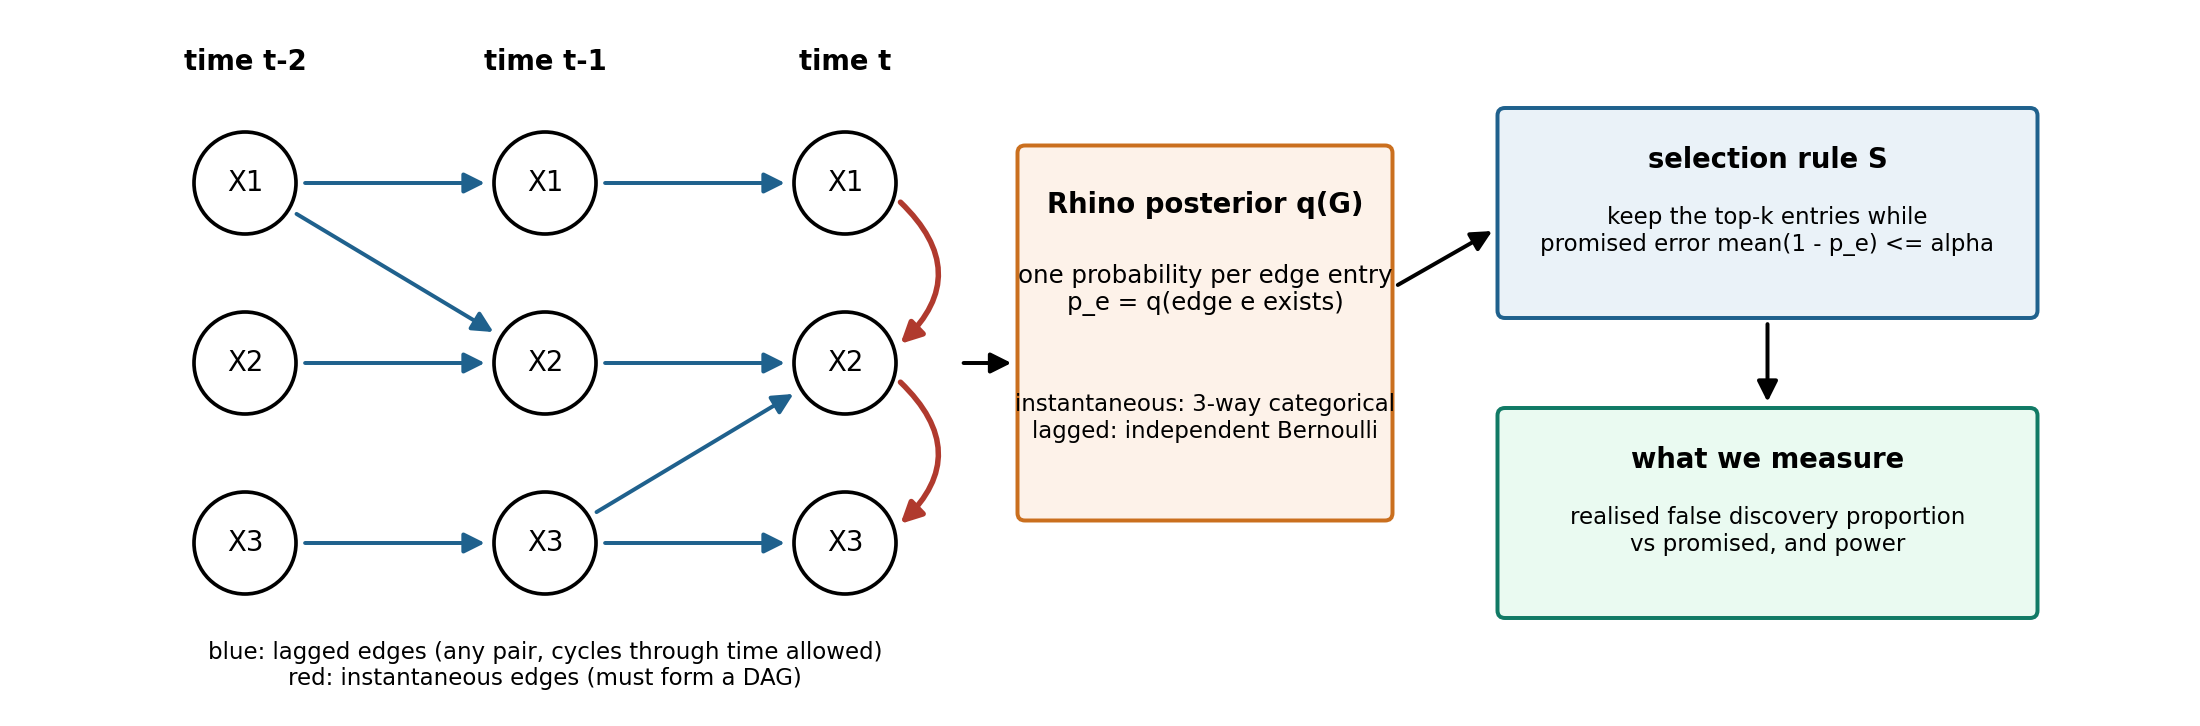
\includegraphics[width=0.98\textwidth]{figures/fig_model.png}
\captionsetup{type=figure}\caption*{\textbf{Figure 2:} Left, the temporal graph that Rhino models (three variables, lag 2). Middle, the posterior q(G) over its edges. Right, the selection layer added in this work.}
\end{figure}
\textbf{Variables and nodes.} The nodes are the D observed variables at each time step. An edge entry (l, i, j) means that variable i at time t $-$ l is a direct cause of variable j at time t.

\textbf{Factorization.} Given a graph $G$, the data follow

\begin{equation}p(X_t\mid X_{<t},G)=\prod_{i=1}^{D}p\big(x_{i,t}\mid \mathrm{Pa}_i^{<t},\mathrm{Pa}_i^{t},G\big).\end{equation}
Each variable depends on its parents only. So $x_{i,t}$ is conditionally independent of its non-parents given its parents. The instantaneous slice must be acyclic. The lagged slices may contain any pattern, since time orders them.

\textbf{The posterior as a second graphical model.} The posterior over graphs factorises as a product over node pairs and lags. For each pair (i, j) with i > j the instantaneous part is one categorical variable with three states: edge from j to i, edge from i to j, or no edge. For each lag l $\ge$ 1 and each (i, j) the lagged part is an independent Bernoulli variable (Gong et al., 2023). This product form matters for my argument. The marginal probability of each entry is a simple function of the learned logits, so I can read it exactly (Section 8). The product form is also wrong in one respect: it ignores dependencies between edges, which the acyclicity penalty creates during training.

\textbf{Why a PGM is appropriate.} The directed graph states which variables influence which, and the factorization turns this into a likelihood. The posterior over graphs turns structure learning into inference, and this is why a calibration question can be asked at all. A method that returns a single graph has no probabilities to check.

\section{Learning Method}
\textbf{Parameter and structure learning in Rhino.} Rhino maximises the evidence lower bound

\begin{equation}\mathrm{ELBO}=\mathbb{E}_{q(G)}\Big[\sum_{n}\log p(X_n\mid G)+\log p(G)\Big]+H\big(q(G)\big).\end{equation}
The prior $p(G)$ rewards sparse graphs with a weight $\lambda_s$. An acyclicity penalty $h(G)=\mathrm{tr}\,\exp(G\circ G)-D$ (Zheng et al., 2018) acts on the instantaneous part, and its weight grows in steps of an augmented Lagrangian method. Graph samples use the Gumbel-softmax estimator. The number of augmented Lagrangian steps is the training length. I did not retrain. I use the models of M3: Rhino with the settings printed in the paper ($\lambda_s=9$, lag 2), Rhino+g, Rhino+s, and Rhino with the released configuration.

\textbf{What I learn in this report.} Two things, both on top of the frozen posterior, and both with labelled calibration data:

\begin{itemize}
\item \textbf{Temperature.} p' = sigmoid(logit(p) / $\tau$). One parameter, fitted by minimising log-loss on pooled entries of the calibration datasets. The fit uses grouped 5-fold cross-validation over datasets, so a dataset never helps to fit the $\tau$ that is applied to it (numpy seed 0). Mean $\tau$ = 5.23 (SD 0.17).
\item \textbf{Cutoff.} For each budget $\alpha$, find on the pooled calibration entries the lowest score cutoff (on the log-odds) so that the selected entries have FDP at most $\alpha$. Cutoffs are placed only between distinct score values. A cutoff needs at least 10 entries. If no cutoff exists the rule selects nothing. One variant pools all calibration datasets. The other uses only datasets with the same number of nodes (it falls back to pooling if there are none).
\end{itemize}
\textbf{Why these choices.} Temperature scaling is the standard single-parameter fix and it keeps the ranking (Guo et al., 2017). The cutoff rule is the simplest direct way to hit a target FDP on average. It is the empirical version of choosing a parameter for risk control (Angelopoulos et al., 2021), without the finite-sample guarantee.

\section{Inference Method}
\textbf{What is inferred.} The marginal probability $p_{e}$ of every edge entry, and from it a selected set S. These are the quantities a user would read from the posterior.

\textbf{Exact marginals.} The saved weights hold the logits of q(G). For an instantaneous pair (i > j), p(j to i), p(i to j) and p(no edge) are the softmax of the three logits. For a lagged entry, p = softmax(logits\_lag)(Gong et al., 2023). For data sets whose truth is an aggregated graph (Netsim, DREAM3), the entry (i, j) is an edge if it exists at any lag, so p = 1 $-$ product over lags of (1 $-$ p\_l). This is exact under q, because the lags are independent. I check this against the mean of the 100 graphs that the official code saves. The mean absolute difference is 0.0067 over all entries of the 760 exported runs (the largest per-run mean is 0.0297, and the largest single difference is 0.206). The largest value is what 100 samples give by chance over about a million entries, and a wrong mapping would give much larger differences.

\textbf{Why exact and not sampled.} 100 samples give a resolution of 0.01 and many ties at 0 and 1. Exact values break the ties and show how far the saturation goes. I report the sampled version as a robustness check (Appendix C). The conclusions do not change.

\textbf{Bayesian FDR selection.} Sort the entries by p, take cumulative means of (1 $-$ p) and keep the largest top-k with mean at most $\alpha$. This takes O(E log E) time for E entries, which is negligible. The cost of the whole approach is the training of the model, which in M3 was about 170 times that of PCMCI+ at 20 nodes.

\section{Experimental Setup}
\textbf{Data and models.} All runs are the finished runs of M3 [Appendix C]. Synthetic: the authors' generator (Microsoft, 2022), 5, 10 and 20 nodes, graph family ER or SF, with or without instantaneous effects, with or without history-dependent noise, data seeds 0 to 4, 40 datasets per dimension, 120 datasets per method. One model seed per dataset. Rhino, Rhino+g and Rhino+s run on all 120. The released configuration of Rhino ran on 80. A dataset has 70, 290 or 1,180 edge entries (3 N\textasciicircum{}2 $-$ N for N = 5, 10, 20), so the 120 Rhino datasets give 61600 entries. Real: Netsim Sim-3 (15 regions, 5 runs per setting) and DREAM3 size 100 (5 networks, 5 seeds). Truth for Netsim and DREAM3 is an aggregated graph.

\textbf{Protocol.} (1) Read the exact p of each run and the true graph. (2) For the synthetic runs, fit the calibration on 4/5 of the datasets and apply it to the other 1/5, five times. (3) For the real data, fit on all synthetic Rhino runs and apply to the real runs, which tests a shift of distribution. (4) Compute all KPIs per dataset. I do not change any condition between methods. Hardware and software: M3 runs used Windows 11, Python 3.9, torch 1.12.1 on CPU. The analysis of this report runs on Python 3.14 with numpy 2.4.2, scipy 1.17.1, pandas 3.0.1 and scikit-learn 1.9.0. Commands and seeds are in Code/README.md.

\textbf{Statistics.} Mean and standard deviation over datasets. 95\% intervals from the t distribution, except the pooled ECE, which uses a bootstrap over datasets (1000 resamples, seed 0). Paired comparisons use the Wilcoxon signed-rank test (Wilcoxon, 1945) with the Holm correction (Holm, 1979).

\section{Baselines}
\begin{table}[!ht]\centering
\captionsetup{type=table}\caption*{\textbf{Table 3:} Selection rules compared (same data, same folds)}
\footnotesize
\begin{tabular}{>{\raggedright\arraybackslash}p{1.45in}>{\raggedright\arraybackslash}p{2.98in}>{\raggedright\arraybackslash}p{0.80in}}\toprule
\textbf{Rule} & \textbf{How it chooses the edge set} & \textbf{Uses labels?} \\ \midrule
Raw, threshold 0.5 & Round q(G) at 0.5. This is how Rhino's graph is read in the paper & No \\
Raw, Bayesian FDR & Largest top-k with mean(1 $-$ p) $\le$ $\alpha$, using Rhino's p as given & No \\
Temperature, Bayesian FDR & Same, after p' = sigmoid(logit(p)/$\tau$), $\tau$ from other datasets & Calibration datasets \\
Temperature, expected F1 & Top-k that maximises 2 sum(p') / (k + sum of all p') & Calibration datasets \\
Learned cutoff (pooled, or same size) & Log-odds cutoff with pooled FDP $\le$ $\alpha$ on other datasets & Calibration datasets \\
Oracle threshold & Best F1 over all thresholds, using the truth. An upper bound, not usable & Truth of the test dataset \\
\bottomrule\end{tabular}
\end{table}
The first two rows are the practice that the paper suggests. The oracle is a ceiling. M3 compared Rhino with PCMCI+, DYNOTEARS and VAR-LiNGAM on accuracy. These methods return no probabilities, so they cannot take part in a calibration comparison. I use Rhino+g and Rhino+s as comparators, since they change only the noise model.

\section{KPIs}
\begin{table}[!ht]\centering
\captionsetup{type=table}\caption*{\textbf{Table 4:} KPIs and why each one is used}
\footnotesize
\begin{tabular}{>{\raggedright\arraybackslash}p{0.71in}>{\raggedright\arraybackslash}p{1.58in}>{\raggedright\arraybackslash}p{1.66in}>{\raggedright\arraybackslash}p{1.19in}}\toprule
\textbf{Layer} & \textbf{KPI} & \textbf{Why} & \textbf{Caveat} \\ \midrule
Representation & Share of entries with p < 0.001 or > 0.999. Edge rate in each group & Shows how saturated the posterior is, and how often certainty is wrong & Depends on the 0.001 cut \\
Learning & Brier score, log-loss, pooled ECE (10 bins) & Probability quality, as the course asks & ECE is small when edges are rare, even for bad rankings \\
Learning & $\tau$ (fitted temperature) & Size of the overconfidence in one number & Single global value \\
Inference & Realised FDP against budget $\alpha$, promised error, empty-set rate & Direct test of the claim `at most $\alpha$ wrong' & Empty set counts as FDP 0, so power must be read with it \\
Inference & Power (recall of true edges) & Price of control & Needs the truth \\
Structure & AUROC, AUPRC, F1 at 0.5, oracle F1 & Quality of the ranking and of the graph & AUROC pools entries per dataset \\
Cost & Training time (M3), selection time & Practical cost & CPU only \\
\bottomrule\end{tabular}
\end{table}
\section{Results}
These results are a first test of the plan in Section 2.5 on finished M3 runs. They are one benchmark family, one model seed per dataset, and a small real-data part. I read them as early evidence for the idea and not as a validation of it.

\subsection{The posterior is saturated}
Over 61600 synthetic entries of Rhino, 46.1\% have p below 0.001 and 9.4\% have p above 0.999. Only a small part lies in between. Among the entries that Rhino calls certainly absent, 17.6\% are true edges. Among the entries it calls certainly present, 23.3\% are not edges (Fig. 3, Table 5).

\begin{figure}[!ht]\centering
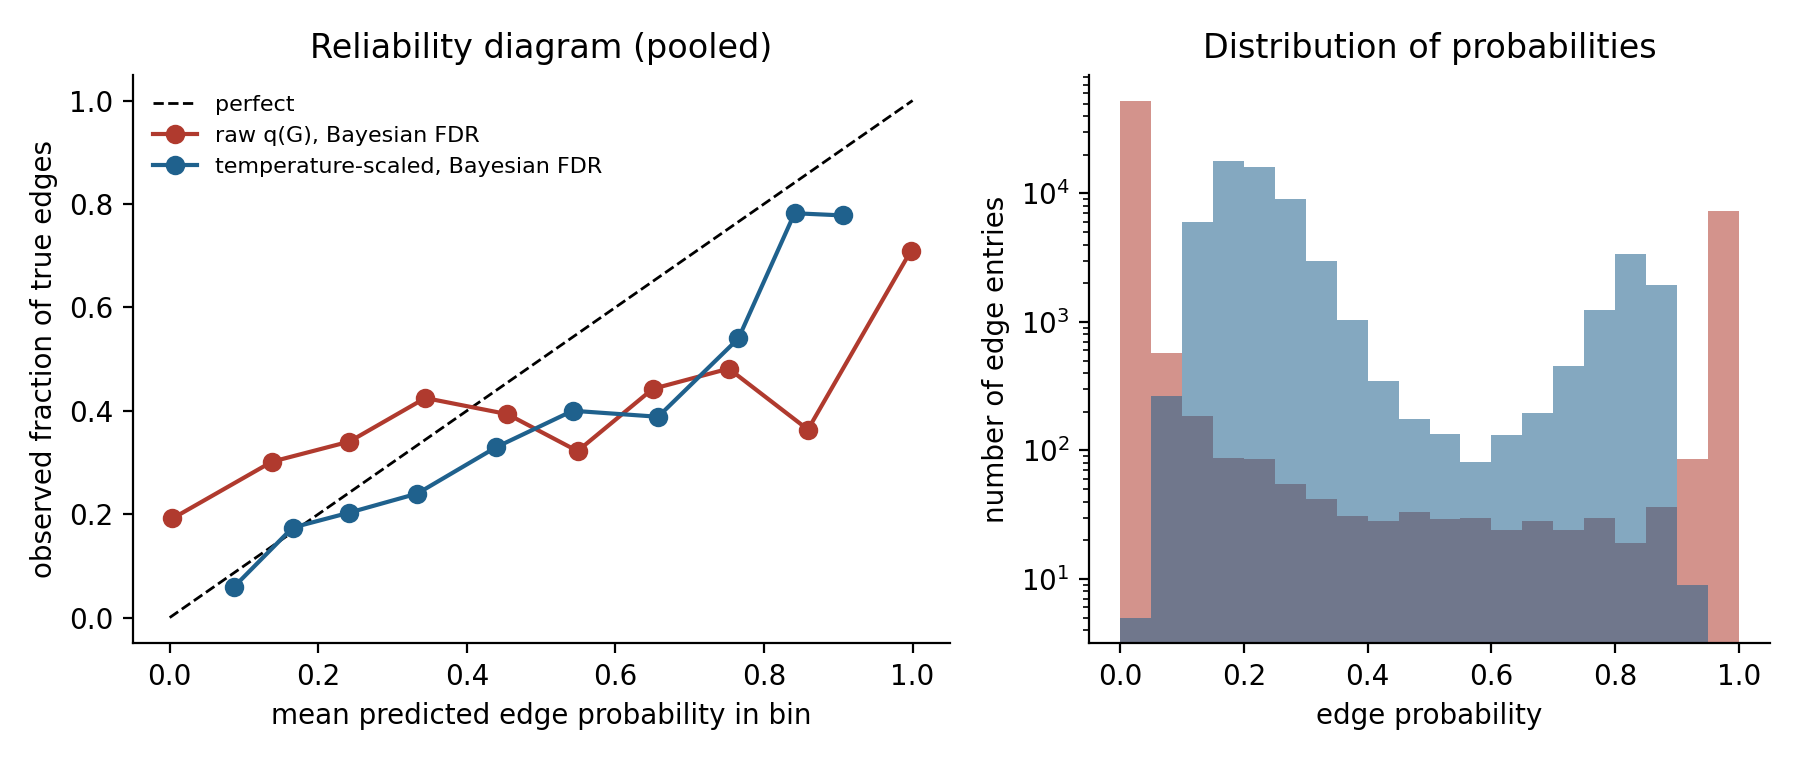
\includegraphics[width=0.95\textwidth]{figures/fig_reliability_synth_rhino_exact.png}
\captionsetup{type=figure}\caption*{\textbf{Figure 3:} Left, reliability diagram, pooled over 120 synthetic datasets, exact probabilities. Right, histogram of the probabilities (log scale).}
\end{figure}
\begin{table}[!ht]\centering
\captionsetup{type=table}\caption*{\textbf{Table 5:} Probability quality, Rhino (paper settings), 120 synthetic datasets}
\footnotesize
\begin{tabular}{>{\raggedright\arraybackslash}p{0.91in}>{\raggedright\arraybackslash}p{1.14in}>{\raggedright\arraybackslash}p{0.53in}>{\raggedright\arraybackslash}p{0.61in}>{\raggedright\arraybackslash}p{0.91in}>{\raggedright\arraybackslash}p{0.38in}>{\raggedright\arraybackslash}p{0.38in}}\toprule
\textbf{Variant} & \textbf{Pooled ECE [95\% CI]} & \textbf{Brier (pooled)} & \textbf{Log-loss (pooled)} & \textbf{Brier, mean $\pm$ SD over datasets} & \textbf{AUROC} & \textbf{AUPRC} \\ \midrule
Raw q(G) & 0.200 [0.169, 0.232] & 0.203 & 1.39 & 0.207 $\pm$ 0.117 & 0.724 & 0.609 \\
Temperature scaled & 0.039 [0.022, 0.067] & 0.163 & 0.51 & 0.166 $\pm$ 0.069 & 0.724 & 0.609 \\
\bottomrule\end{tabular}
\par\vspace{3pt}{\footnotesize Log-loss clips probabilities at 1e-6. AUROC and AUPRC are means over datasets and are identical for both rows because temperature scaling keeps the ranking (Proposition 3).}
\end{table}
\textbf{What happened.} Rhino's probabilities are close to 0 or 1 and both kinds of certainty are often wrong. \textbf{Was it expected?} Partly. M3 showed that training makes the posterior more confident. \textbf{Why?} The variational posterior is trained to maximise the likelihood of the data, and the acyclicity penalty and the entropy term push the logits apart as the number of augmented Lagrangian steps grows. I did not isolate the cause, and Section 12.7 gives indirect evidence only. \textbf{What it tells us.} The posterior does not report uncertainty about the graph in a usable way.

\subsection{The trust gap: promised and realised error}
At a budget of 0.01 the raw posterior promises an error of 0.004. The realised FDP is 0.306 [0.277, 0.335]. At a budget of 0.1 it is 0.351 [0.323, 0.379], and at 0.2 it is 0.398 [0.371, 0.425]. So H1 is supported. By the identity of Section 2.3, the gap equals the overconfidence of the posterior on the selected set. The sampled estimate of p (100 graphs) gives the same result: 0.306 [0.277, 0.335] at a budget of 0.01.

The dependence on the data is strong (Table 6). Rhino is much better when the noise is history-dependent, which is the case it was designed for, and worse when the graph is larger. For example, at 5 nodes with history-dependent noise the realised FDP at budget 0.1 is 0.216 and the AUROC is 0.861. At 20 nodes without history-dependent noise they are 0.520 and 0.573.

\begin{table}[!ht]\centering
\captionsetup{type=table}\caption*{\textbf{Table 6:} Rhino (paper settings) by dataset type, exact probabilities, 20 datasets per row}
\footnotesize
\begin{tabular}{>{\raggedright\arraybackslash}p{0.45in}>{\raggedright\arraybackslash}p{0.97in}>{\raggedright\arraybackslash}p{0.52in}>{\raggedright\arraybackslash}p{0.52in}>{\raggedright\arraybackslash}p{0.60in}>{\raggedright\arraybackslash}p{0.60in}>{\raggedright\arraybackslash}p{1.20in}}\toprule
\textbf{Nodes} & \textbf{History-dependent noise} & \textbf{AUROC} & \textbf{Brier} & \textbf{F1 at 0.5} & \textbf{Oracle F1} & \textbf{Realised FDP at budget 0.1 (raw)} \\ \midrule
5 & no & 0.669 & 0.275 & 0.568 & 0.645 & 0.387 \\
5 & yes & 0.861 & 0.154 & 0.767 & 0.807 & 0.216 \\
10 & no & 0.629 & 0.250 & 0.453 & 0.549 & 0.458 \\
10 & yes & 0.821 & 0.164 & 0.658 & 0.711 & 0.258 \\
20 & no & 0.573 & 0.239 & 0.283 & 0.472 & 0.520 \\
20 & yes & 0.793 & 0.163 & 0.599 & 0.668 & 0.269 \\
\bottomrule\end{tabular}
\par\vspace{3pt}{\footnotesize F1 is computed over all temporal edge entries. It matches the orientation F1 of the M3 report (0.67, 0.55, 0.44 at 5, 10, 20 nodes), which shows that the export reads the same graphs.}
\end{table}
\subsection{Temperature scaling repairs the scores, not the error control}
The fitted temperature is 5.23 (SD 0.17 over folds). It lowers the pooled ECE from 0.200 to 0.039, the pooled Brier score from 0.203 to 0.163, and the pooled log-loss from 1.39 to 0.51 (Table 5). The per-dataset differences are significant (Table 10). But error control is not restored (Table 7, Fig. 4). At budgets of 0.01 and 0.05 the rule selects no edges at all. At 0.1 it selects edges in 6.7\% of the datasets. At 0.2 it promises 0.195, and the realised FDP is 0.314 [0.287, 0.340]. So H2 is supported for the scores and not supported for error control. \textbf{Why.} ECE and log-loss measure the average match over all entries, and most entries are easy ones with p near 0. Error control depends on the match in the top of the ranking, and this part stays overconfident. A better ECE is therefore a poor guide to whether the selected edges are reliable.

\subsection{A cutoff learned on other datasets}
The learned cutoff (pooled) gives a realised FDP of 0.062 [0.031, 0.093] at budget 0.1, 0.244 [0.217, 0.270] at 0.2 and 0.311 [0.281, 0.341] at 0.3. The same-size variant gives 0.088 [0.051, 0.126], 0.228 [0.198, 0.258] and 0.321 [0.292, 0.351]. At budgets of 0.1 and 0.3 the intervals contain or lie below the budget. At 0.2 the pooled cutoff is above it (interval 0.217 to 0.270) and the same-size cutoff contains it, so control is approximate and not exact. The price is power: 0.026 at 0.1, 0.369 at 0.2 and 0.499 at 0.3, and at budget 0.1 the rule selects nothing in 43.3\% of the datasets. Compared with the raw rule, which has 0.532 power at budget 0.2 but a realised FDP of 0.398, the learned cutoff gives up power to keep its promise.

\begin{figure}[!ht]\centering
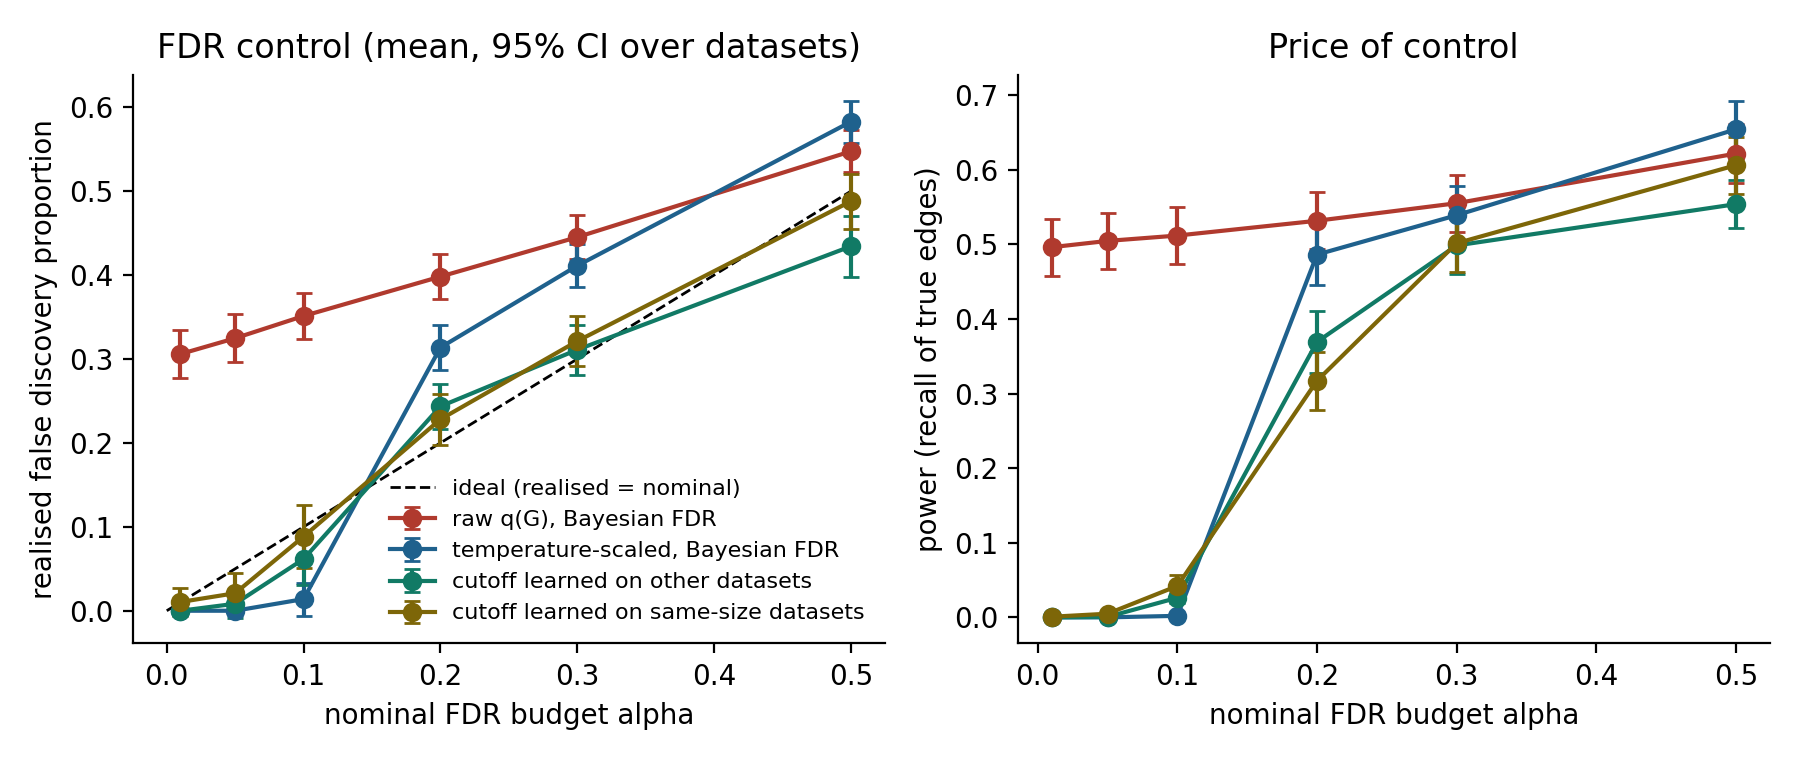
\includegraphics[width=0.98\textwidth]{figures/fig_fdr_control_synth_rhino_exact.png}
\captionsetup{type=figure}\caption*{\textbf{Figure 4:} Realised false discovery proportion (left) and power (right) against the nominal budget, Rhino (paper settings), 120 datasets, exact probabilities. Bars: 95\% t intervals over datasets.}
\end{figure}
\begin{table}[!ht]\centering
\captionsetup{type=table}\caption*{\textbf{Table 7:} Error control at budget $\alpha$: realised FDP [95\% CI] and power / share of datasets with an empty selection}
\scriptsize
\begin{tabular}{>{\raggedright\arraybackslash}p{0.31in}>{\raggedright\arraybackslash}p{0.47in}>{\raggedright\arraybackslash}p{0.82in}>{\raggedright\arraybackslash}p{0.39in}>{\raggedright\arraybackslash}p{0.82in}>{\raggedright\arraybackslash}p{0.58in}>{\raggedright\arraybackslash}p{0.82in}>{\raggedright\arraybackslash}p{0.58in}}\toprule
\textbf{$\alpha$} & \textbf{Raw: promised} & \textbf{Raw: realised} & \textbf{Raw: power} & \textbf{Temperature: realised} & \textbf{Temp.: power / empty} & \textbf{Learned cutoff: realised} & \textbf{Cutoff: power / empty} \\ \midrule
0.05 & 0.039 & 0.325 [0.296, 0.354] & 0.505 & 0.000 [0.000, 0.000] & 0.000 / 100.0\% & 0.008 [-0.008, 0.025] & 0.001 / 97.5\% \\
0.1 & 0.091 & 0.351 [0.323, 0.379] & 0.512 & 0.014 [-0.006, 0.034] & 0.002 / 93.3\% & 0.062 [0.031, 0.093] & 0.026 / 43.3\% \\
0.2 & 0.192 & 0.398 [0.371, 0.425] & 0.532 & 0.314 [0.287, 0.340] & 0.486 / 0.0\% & 0.244 [0.217, 0.270] & 0.369 / 0.8\% \\
0.3 & 0.293 & 0.445 [0.419, 0.471] & 0.555 & 0.411 [0.386, 0.437] & 0.539 / 0.0\% & 0.311 [0.281, 0.341] & 0.499 / 0.0\% \\
\bottomrule\end{tabular}
\par\vspace{3pt}{\footnotesize An empty selection counts as FDP = 0. The shares of empty selections show how much of a low realised FDP comes from selecting nothing.}
\end{table}
\textbf{Reading.} The H5 result is mixed. The learned cutoff keeps the error near the budget for budgets of 0.1 to 0.3, but at budgets of 0.05 or lower it has almost no power. For this benchmark the smallest useful budget is about 0.1. Section 12.7 shows that this does not hold on real data. H5 was added after the H2 result, so it is an exploratory finding.

\subsection{Choosing a graph: the expected-F1 rule}
After temperature scaling, the graph that maximises the expected F1 under the posterior gives an F1 of 0.522. A threshold of 0.5 gives 0.555, and the oracle threshold gives 0.642. The paired difference to the 0.5 threshold is -0.033 [-0.059, -0.006] (Holm p = 0.004). So H3 is not supported: the label-free rule is slightly worse than a plain threshold, and even the plain threshold is about 0.09 below the oracle. \textbf{Why.} The rule needs the probabilities to be calibrated in the region that decides the F1, and temperature scaling does not give this (Section 12.3). \textbf{What it tells us.} The gap to the oracle is the value of knowing the right threshold for each dataset. The paper tunes the threshold on DREAM3 with the truth, which hides this gap.

\subsection{Accuracy against trust across the Rhino variants}
\begin{table}[!ht]\centering
\captionsetup{type=table}\caption*{\textbf{Table 8:} Variants of Rhino, exact probabilities (budget 0.1 for the raw rule, budget 0.2 for the learned cutoff)}
\scriptsize
\begin{tabular}{>{\raggedright\arraybackslash}p{0.87in}>{\raggedright\arraybackslash}p{0.29in}>{\raggedright\arraybackslash}p{0.44in}>{\raggedright\arraybackslash}p{0.36in}>{\raggedright\arraybackslash}p{0.40in}>{\raggedright\arraybackslash}p{0.36in}>{\raggedright\arraybackslash}p{0.33in}>{\raggedright\arraybackslash}p{0.36in}>{\raggedright\arraybackslash}p{0.36in}>{\raggedright\arraybackslash}p{0.36in}>{\raggedright\arraybackslash}p{0.36in}}\toprule
\textbf{Variant} & \textbf{Runs} & \textbf{AUROC} & \textbf{F1 (0.5)} & \textbf{Wrong at p > 0.999} & \textbf{Share p > 0.999} & \textbf{ECE} & \textbf{Raw FDP (0.1)} & \textbf{Raw power (0.1)} & \textbf{Cutoff FDP (0.2)} & \textbf{Cutoff power (0.2)} \\ \midrule
Rhino (paper settings) & 120 & 0.724 & 0.555 & 23.3\% & 9.4\% & 0.200 & 0.351 & 0.512 & 0.244 & 0.369 \\
Rhino+g (Gaussian noise) & 120 & 0.693 & 0.461 & 40.6\% & 7.1\% & 0.196 & 0.449 & 0.443 & 0.017 & 0.000 \\
Rhino+s (spline noise, no history) & 120 & 0.675 & 0.267 & 10.8\% & 2.3\% & 0.208 & 0.103 & 0.204 & 0.124 & 0.211 \\
Rhino (released config) & 80 & 0.739 & 0.603 & 40.7\% & 25.8\% & 0.249 & 0.434 & 0.664 & 0.079 & 0.014 \\
\bottomrule\end{tabular}
\par\vspace{3pt}{\footnotesize Rhino (released config) has 80 runs on a different subset of datasets. It is not paired with the other rows.}
\end{table}
Rhino has the best ranking and the best F1 of the variants that ran on all 120 datasets (AUROC 0.724, F1 0.555). Its trust is poor (0.351 realised at a budget of 0.1), and Rhino+g is worse (0.449). Rhino+s has a weaker ranking (AUROC 0.675) and much lower F1 (0.267), but its raw posterior is close to its promise: 0.103 realised at a budget of 0.1. Many of its selections are empty (43.3\% of the datasets at budget 0.1), so part of this is selecting little. I read this as an accuracy against trust trade-off between the noise models. I do not claim a cause. A model that fits the noise more flexibly may also produce a more saturated posterior. I did not test this.

\subsection{Real data and the shift of distribution}
\begin{table}[!ht]\centering
\captionsetup{type=table}\caption*{\textbf{Table 9:} Real data. Tau and cutoffs are fitted on the synthetic Rhino runs only. Raw rule at budget 0.1, temperature and cutoff at budget 0.2}
\scriptsize
\begin{tabular}{>{\raggedright\arraybackslash}p{1.02in}>{\raggedright\arraybackslash}p{0.35in}>{\raggedright\arraybackslash}p{0.51in}>{\raggedright\arraybackslash}p{0.47in}>{\raggedright\arraybackslash}p{0.47in}>{\raggedright\arraybackslash}p{0.47in}>{\raggedright\arraybackslash}p{0.47in}>{\raggedright\arraybackslash}p{0.47in}>{\raggedright\arraybackslash}p{0.47in}}\toprule
\textbf{Data} & \textbf{Runs} & \textbf{AUROC} & \textbf{Raw FDP (0.1)} & \textbf{Raw power (0.1)} & \textbf{Temp. FDP (0.2)} & \textbf{Temp. power (0.2)} & \textbf{Cutoff FDP (0.2)} & \textbf{Cutoff power (0.2)} \\ \midrule
Netsim, paper steps & 5 & 0.985 & 0.137 & 0.758 & 0.000 & 0.000 & 0.000 & 0.000 \\
Netsim, released config & 5 & 0.949 & 0.349 & 0.933 & 0.310 & 0.848 & 0.053 & 0.527 \\
DREAM3, Rhino & 25 & 0.604 & 0.859 & 0.114 & 0.883 & 0.092 & 0.980 & 0.010 \\
DREAM3, Rhino+g & 25 & 0.606 & 0.845 & 0.126 & 0.877 & 0.084 & 0.985 & 0.006 \\
\bottomrule\end{tabular}
\par\vspace{3pt}{\footnotesize Netsim has 5 runs per setting, so intervals are wide and I report means only. DREAM3 has 25 runs (5 networks times 5 seeds).}
\end{table}
On Netsim with the paper's training steps, the raw posterior is close to its promise (0.137 realised at budget 0.1). With the released configuration, which trains for a different number of augmented Lagrangian steps, it is not (0.349). The two settings differ in more than the number of steps that I could isolate, and each has 5 runs. This is indirect evidence for the link between training length and overconfidence, and no more than that. On the synthetic runs, the released configuration has more entries with p above 0.999 (25.8\% against 9.4\%) and a higher ECE (0.249 against 0.200), which points in the same direction.

On DREAM3 the method fails. The AUROC is 0.604, and 85.9\% of the edges selected at budget 0.1 are wrong. The temperature and the cutoffs from synthetic data do not help: the learned cutoff gives a realised FDP of 0.980 at budget 0.2. The temperature fitted on synthetic data also does not transfer to Netsim: with the paper's steps it is too strong and the rule selects nothing, even at budget 0.2 (Table 9). So H4 holds in its second form: the guarantee does not transfer, and it degrades in line with Proposition 2. When the ranking is poor (DREAM3), no calibration can help (Proposition 3).

\section{Statistical Analysis}
\begin{table}[!ht]\centering
\captionsetup{type=table}\caption*{\textbf{Table 10:} Paired comparisons over the 120 synthetic datasets (mean difference [95\% t interval], wins / losses, Holm-corrected Wilcoxon p)}
\footnotesize
\begin{tabular}{>{\raggedright\arraybackslash}p{2.61in}>{\raggedright\arraybackslash}p{1.34in}>{\raggedright\arraybackslash}p{0.63in}>{\raggedright\arraybackslash}p{0.55in}}\toprule
\textbf{Quantity (second method minus first)} & \textbf{Mean difference [95\% CI]} & \textbf{Wins / losses} & \textbf{p (Holm)} \\ \midrule
Brier & -0.041 [-0.050, -0.033] & 91 / 29 & <0.001 \\
log-loss & -0.993 [-1.115, -0.871] & 117 / 3 & <0.001 \\
ECE (per dataset) & -0.065 [-0.086, -0.045] & 80 / 40 & <0.001 \\
F1, expected-F1 rule (vs threshold 0.5) & -0.033 [-0.059, -0.006] & 34 / 60 & 0.004 \\
|FDP $-$ $\alpha$|, $\alpha$ = 0.1: learned cutoff minus raw & -0.122 [-0.155, -0.088] & 88 / 28 & <0.001 \\
|FDP $-$ $\alpha$|, $\alpha$ = 0.1: learned cutoff minus temperature & +0.021 [-0.002, +0.044] & 2 / 12 & 0.016 \\
|FDP $-$ $\alpha$|, $\alpha$ = 0.2: learned cutoff minus raw & -0.083 [-0.106, -0.059] & 89 / 31 & <0.001 \\
|FDP $-$ $\alpha$|, $\alpha$ = 0.2: learned cutoff minus temperature & -0.023 [-0.039, -0.008] & 71 / 47 & 0.014 \\
\bottomrule\end{tabular}
\par\vspace{3pt}{\footnotesize For Brier, log-loss, ECE and |FDP $-$ $\alpha$| a negative difference is better for the second method. Wins are counted in favour of the second method, and ties are not counted. For the F1 row, the difference is the expected-F1 rule minus the 0.5 threshold, after temperature scaling.}
\end{table}
\textbf{Reading.} Temperature scaling improves the Brier score, the log-loss and the ECE on most datasets, and the differences are far from zero. The learned cutoff is much closer to the budget than the raw rule at both budgets. Against temperature scaling the answer depends on the budget. At 0.1 both rules select nothing on most datasets, so most comparisons are ties, and the cutoff is slightly farther from the budget (+0.021, interval touching zero). At 0.2 the cutoff is closer (-0.023, 71 wins against 47 losses). I applied the Holm correction within this family of tests. \textbf{Sources of uncertainty.} The intervals show spread over datasets. Each dataset has one model seed, so I cannot separate dataset spread from training noise. The Netsim comparisons rest on 5 runs, and the DREAM3 numbers on 25 runs from 5 networks, so they are not independent. The bootstrap interval of the ECE resamples datasets, not entries.

\begin{table}[!ht]\centering
\captionsetup{type=table}\caption*{\textbf{Table 11:} Expectations and outcomes}
\footnotesize
\begin{tabular}{>{\raggedright\arraybackslash}p{1.77in}>{\raggedright\arraybackslash}p{1.29in}>{\raggedright\arraybackslash}p{2.17in}}\toprule
\textbf{Hypothesis} & \textbf{Outcome} & \textbf{Evidence} \\ \midrule
H1 raw posterior breaks its budget & Supported & Realised FDP 0.306 at budget 0.01 and 0.351 at 0.1, intervals far above the budget \\
H2 temperature fixes scores and control & Scores: supported. Control: not supported & ECE 0.200 to 0.039. FDP at 0.2 is 0.314 against 0.195 promised \\
H3 expected-F1 rule beats threshold 0.5 & Not supported & F1 0.522 against 0.555 \\
H4 $\tau$ transfers to real data, or degrades as predicted & Does not transfer. Degrades as predicted & Netsim over-corrected, DREAM3 fails because the ranking is weak \\
H5 learned cutoff gives FDP near $\alpha$ (exploratory) & Partly supported & Within or near the budget for 0.1 to 0.3 on synthetic data. Power 0.026 to 0.499. Fails on DREAM3 \\
\bottomrule\end{tabular}
\end{table}
\section{Discussion}
\textbf{What the results mean.} A Bayesian graph posterior is only useful for error control if it is calibrated where the decisions are made. Rhino's is not. It is saturated, and the certainty is often wrong. The identity of Section 2.3 reads the failure in one line: the realised error is the promised error plus the overconfidence on the selected set. Standard calibration reduces the average overconfidence and leaves the part in the top of the ranking. That is why the ECE drops by a factor of five while the realised FDP at budget 0.2 stays 0.12 above the promise.

\textbf{What works, and when.} A cutoff learned on similar datasets gives approximate control for moderate budgets, and it needs no change of the model. It works because it uses the labels exactly where the decision is made. It fails when the calibration data do not resemble the new data (DREAM3, and partly Netsim) and when the ranking is weak.

\textbf{Benefits and costs for a practitioner.} Benefit: one can state a budget and get a list, at a small and known price in power. Cost: one needs labelled graphs from a similar setting, the guarantee is on average and not per dataset, and for small budgets the list is empty. In a field where no such labelled data exist (most real applications), the honest advice from this study is to treat Rhino's probabilities as a ranking and not as probabilities.

\textbf{What I learned.} Reproducing a paper is not enough to say that its output can be used. The accuracy ranking of the variants and their trust ranking differ. A good-looking calibration metric can hide a failure in the part of the ranking that matters. The metrics chosen at the start (realised FDP against budget) were the ones that exposed this.

\textbf{Revisiting M1 and M2.} The research question of M1 and M2 was about uGLAD. It is replaced here. What survived is the KPI discipline (precision, recall, F1, SHD), the habit of checking my own implementation against the authors' output, and the habit of reporting what did not reproduce. M3 reproduced the base paper, and this report asks a question that it did not ask.

\section{Limitations}
\begin{itemize}
\item \textbf{Average guarantee only.} The cutoff controls the expected FDP over datasets like the calibration datasets. It gives no finite-sample guarantee and no per-dataset guarantee. A method such as Learn then Test (Angelopoulos et al., 2021) would give a finite-sample bound. I did not implement it.
\item \textbf{Needs labelled graphs} from similar data. This is the main practical cost.
\item \textbf{Transfer fails} from synthetic to DREAM3, and partly to Netsim. Netsim has 5 runs per setting.
\item \textbf{Weak ranking limits everything.} Calibration cannot repair it (Proposition 3).
\item \textbf{Training length is only indirectly tested.} The comparison of paper and released settings is confounded, and the runs are few. I did not run a controlled sweep of the number of steps.
\item \textbf{One model seed per dataset.} I cannot separate training noise from dataset variation.
\item \textbf{Scope.} 5, 10 and 20 nodes, one family of models, no 40-node runs. No missing data, no hidden confounders and no non-stationary noise beyond what the model assumes.
\item \textbf{Cycle removal.} I select edge entries without enforcing that the instantaneous part is acyclic. A graph with cycles would need removal of edges, which breaks Proposition 2. I did not measure this.
\item \textbf{Product-form posterior.} Rhino's q(G) ignores dependencies between edges. The identity holds regardless, but the probabilities themselves may be poor for this reason.
\item \textbf{Related work.} The search for earlier work was short. I read the PRCD-MAP paper only in summary.
\end{itemize}
\section{Conclusion}
I asked whether the edge probabilities of Rhino can be trusted for error-controlled selection. In this first test on 500 finished runs the answer is no for the raw posterior: it is saturated and overconfident, and at a budget of 0.01 about 31\% of the selected edges are wrong. Temperature scaling makes the probabilities score well and leaves the error control broken. A cutoff learned on other datasets restores approximate control for budgets of about 0.1 to 0.3, at a large cost in power, and it does not transfer to DREAM3. The identity between promised error, realised error and overconfidence is consistent with each of these outcomes. These are early results on one benchmark family, and they support the idea only within the limits of Section 15.

\textbf{Next research steps.} (1) Replace the learned cutoff by a rule with a finite-sample guarantee. (2) Test the link between training length and saturation with a controlled sweep and a posterior that is regularised against saturation. (3) Use an ensemble over model seeds or a posterior that models dependencies between edges, and see whether the ranking improves. (4) Repeat the audit for other graph posteriors. (5) Extend to 40 nodes, to missing data and to hidden confounders.

\section*{References}
\begingroup\small\setlength{\parskip}{3pt}
\hangindent=0.2in\hangafter=1\noindent A. N. Angelopoulos, S. Bates, E. J. Candès, M. I. Jordan, and L. Lei, ``Learn then Test: Calibrating predictive algorithms to achieve risk control,'' arXiv:2110.01052, 2021.\par
\hangindent=0.2in\hangafter=1\noindent C. K. Assaad, E. Devijver, and E. Gaussier, ``Survey and evaluation of causal discovery methods for time series,'' Journal of Artificial Intelligence Research, vol. 73, pp. 767-819, 2022.\par
\hangindent=0.2in\hangafter=1\noindent Y. Benjamini and Y. Hochberg, ``Controlling the false discovery rate: a practical and powerful approach to multiple testing,'' Journal of the Royal Statistical Society, Series B, vol. 57, no. 1, pp. 289-300, 1995.\par
\hangindent=0.2in\hangafter=1\noindent W. Gong, J. Jennings, C. Zhang, and N. Pawlowski, ``Rhino: Deep Causal Temporal Relationship Learning with History-dependent Noise,'' in International Conference on Learning Representations (ICLR), 2023, arXiv:2210.14706.\par
\hangindent=0.2in\hangafter=1\noindent C. Guo, G. Pleiss, Y. Sun, and K. Q. Weinberger, ``On calibration of modern neural networks,'' in International Conference on Machine Learning (ICML), PMLR 70, pp. 1321-1330, 2017.\par
\hangindent=0.2in\hangafter=1\noindent S. Holm, ``A simple sequentially rejective multiple test procedure,'' Scandinavian Journal of Statistics, vol. 6, no. 2, pp. 65-70, 1979.\par
\hangindent=0.2in\hangafter=1\noindent A. Hyvärinen, K. Zhang, S. Shimizu, and P. O. Hoyer, ``Estimation of a structural vector autoregression model using non-Gaussianity,'' Journal of Machine Learning Research, vol. 11, 2010.\par
\hangindent=0.2in\hangafter=1\noindent F. Jabbari, M. P. Naeini, and G. F. Cooper, ``Obtaining accurate probabilistic causal inference by post-processing calibration,'' arXiv:1712.08626, 2017.\par
\hangindent=0.2in\hangafter=1\noindent S. Khanna and V. Y. F. Tan, ``Economy statistical recurrent units for inferring nonlinear Granger causality,'' arXiv:1911.09879, 2019.\par
\hangindent=0.2in\hangafter=1\noindent L. Lorch, S. Sussex, J. Rothfuss, A. Krause, and B. Schölkopf, ``Amortized inference for causal structure learning,'' in Advances in Neural Information Processing Systems (NeurIPS), vol. 35, pp. 13104-13118, 2022.\par
\hangindent=0.2in\hangafter=1\noindent Microsoft, causica (Rhino code), release v0.0.0, github.com/microsoft/causica/tree/v0.0.0.\par
\hangindent=0.2in\hangafter=1\noindent M. P. Naeini, G. F. Cooper, and M. Hauskrecht, ``Obtaining well calibrated probabilities using Bayesian binning,'' in AAAI Conference on Artificial Intelligence, 2015.\par
\hangindent=0.2in\hangafter=1\noindent M. Nauta, D. Bucur, and C. Seifert, ``Causal discovery with attention-based convolutional neural networks,'' Machine Learning and Knowledge Extraction, vol. 1, no. 1, p. 19, 2019.\par
\hangindent=0.2in\hangafter=1\noindent M. A. Newton, A. Noueiry, D. Sarkar, and P. Ahlquist, ``Detecting differential gene expression with a semiparametric hierarchical mixture method,'' Biostatistics, vol. 5, no. 2, pp. 155-176, 2004.\par
\hangindent=0.2in\hangafter=1\noindent R. Pamfil et al., ``DYNOTEARS: Structure learning from time-series data,'' in International Conference on Artificial Intelligence and Statistics (AISTATS), PMLR, pp. 1595-1605, 2020.\par
\hangindent=0.2in\hangafter=1\noindent B. Guillen Pegueroles, B. Vinzamuri, K. Shanmugam, S. Hedden, J. D. Moyer, and K. R. Varshney, ``Structure learning from time series with false discovery control,'' arXiv:1805.09909, 2018.\par
\hangindent=0.2in\hangafter=1\noindent J. Runge, ``Discovering contemporaneous and lagged causal relations in autocorrelated nonlinear time series datasets,'' in Conference on Uncertainty in Artificial Intelligence (UAI), PMLR, pp. 1388-1397, 2020.\par
\hangindent=0.2in\hangafter=1\noindent X. Shan and D. Zhou, ``PRCD-MAP: Learning how much to trust imperfect priors in causal discovery,'' arXiv:2605.01669, 2026.\par
\hangindent=0.2in\hangafter=1\noindent A. Tank, I. Covert, N. Foti, A. Shojaie, and E. Fox, ``Neural Granger causality for nonlinear time series,'' 2018.\par
\hangindent=0.2in\hangafter=1\noindent F. Wilcoxon, ``Individual comparisons by ranking methods,'' Biometrics Bulletin, vol. 1, no. 6, pp. 80-83, 1945.\par
\hangindent=0.2in\hangafter=1\noindent X. Zheng, B. Aragam, P. Ravikumar, and E. P. Xing, ``DAGs with NO TEARS: Continuous optimization for structure learning,'' in Advances in Neural Information Processing Systems (NeurIPS), vol. 31, 2018.\par
\endgroup
\section*{Appendix A. The identity and two standard facts}
The first item is the identity of Section 2.3. The other two are standard facts that I state for completeness and that the code checks. I do not present them as results of this project.

\textbf{Proposition 1 (identity).} For a non-empty set $S$, $\mathrm{FDP}(S)=\frac{1}{|S|}\sum_{e\in S}(1-y_e)=1-\bar y_S$ and $a(S)=1-\bar p_S$, where the bars are means over $S$. So $\mathrm{FDP}(S)-a(S)=\bar p_S-\bar y_S=o(S)$. This is an identity for any $S$, any dataset and any $p$. The code checks it in tests/test\_calib\_fdr.py.

\textbf{Proposition 2 (control under calibration).} Let $p=(p_e)$ be the vector of forecasts of a dataset and let the set $S=S(p)$ be a function of $p$ only. Assume $\mathbb{E}[y_e\mid p]=p_e$ for every $e$. Then $\mathbb{E}\big[\sum_{e\in S}(1-y_e)\mid p\big]=\sum_{e\in S}(1-p_e)$ by linearity of expectation, since $S$ is fixed given $p$. Dividing by $|S|$ gives $\mathbb{E}[\mathrm{FDP}(S)\mid p]=a(S)$. For $S=S_\alpha$, $a(S)\le\alpha$. If instead $\mathbb{E}[y_e\mid p]\ge p_e-\varepsilon$, the same steps give $\mathbb{E}[\mathrm{FDP}(S)\mid p]\le a(S)+\varepsilon$. No independence between the $y_e$ is used.

\textbf{Proposition 3 (rank invariance).} Let $g$ be strictly increasing and let $p'=g(p)$. The order of entries by $p'$ equals the order by $p$. So the sets of the top-$k$ entries are identical for each $k$, and so are AUROC and AUPRC. Only the mapping from $k$ to the promised error $a(S_k)$ changes.

\textbf{Remark (what is not proved).} The learned cutoff rule has an in-sample guarantee on the pooled calibration entries. I do not prove a bound on the FDP for a new dataset. Section 12.4 is empirical.

\section*{Appendix B. Exact marginals of q(G)}
Let $l_0,l_1,l_2$ be the three logits of an instantaneous pair $(i>j)$ and let $\pi=\mathrm{softmax}(l)$. Then $P(\text{edge from } j \text{ to } i)=\pi_0$, $P(\text{edge from } i \text{ to } j)=\pi_1$ and $P(\text{no edge})=\pi_2$. For a lagged entry with logits $(m_0,m_1)$, $P(\text{edge})=e^{m_1}/(e^{m_0}+e^{m_1})$. The log-odds of an entry are $l_k-\log\sum_{j\ne k}e^{l_j}$, or $m_1-m_0$. I keep the log-odds for the ranking of entries whose probability rounds to 1 in floating point. The code is Code/src/export\_exact\_q.py. A numpy simulation of the same layout agrees with a direct Monte Carlo sampling of the categorical and Bernoulli variables to within 0.002 ($2\times 10^5$ samples, largest difference 0.0016).

\section*{Appendix C. Robustness, reproducibility and files}
\begin{table}[!ht]\centering
\captionsetup{type=table}\caption*{\textbf{Table A1:} Sampled probabilities (100 graphs per run) against exact probabilities, Rhino, 120 datasets}
\footnotesize
\begin{tabular}{>{\raggedright\arraybackslash}p{0.67in}>{\raggedright\arraybackslash}p{0.52in}>{\raggedright\arraybackslash}p{0.52in}>{\raggedright\arraybackslash}p{0.60in}>{\raggedright\arraybackslash}p{0.60in}>{\raggedright\arraybackslash}p{0.97in}>{\raggedright\arraybackslash}p{0.97in}}\toprule
\textbf{Variant} & \textbf{ECE (sampled)} & \textbf{ECE (exact)} & \textbf{Log-loss (sampled)} & \textbf{Log-loss (exact)} & \textbf{Realised FDP at 0.1 (sampled)} & \textbf{Realised FDP at 0.1 (exact)} \\ \midrule
Raw & 0.200 & 0.200 & 2.38 & 1.39 & 0.351 [0.323, 0.379] & 0.351 [0.323, 0.379] \\
Temperature & 0.031 & 0.039 & 0.51 & 0.51 & 0.000 [0.000, 0.000] & 0.014 [-0.006, 0.034] \\
\bottomrule\end{tabular}
\par\vspace{3pt}{\footnotesize The conclusions are the same. The log-loss of the raw posterior differs because sampled values are exactly 0 or 1 more often.}
\end{table}
\textbf{Reproduction.} (1) M3 runs, see M3 folder, Code/README.md. (2) On the workstation, Code/workstation/ builds the two return files: export\_qG.py (100-sample estimate) and export\_exact\_q.py (exact probabilities). (3) python run\_all\_analysis.py --exact, then python run\_all\_analysis.py (Code/src). (4) python make\_model\_figure.py, python build\_report.py. Seeds: the fold split and the bootstrap use numpy seed 0. All tables are in Results/tables, all figures in Results/figures, and the exported probabilities in Results/qG\_export and Results/qG\_exact.

\textbf{Analysed runs.} 760 runs were exported. 500 are analysed here: Rhino 120, Rhino+g 120, Rhino+s 120, Rhino released config 80, Netsim Rhino 10 (two settings), DREAM3 Rhino and Rhino+g 50. The lag ablation runs and Rhino+NoInst on Netsim were exported but not analysed.

\end{document}
